\section{Purpose Definition}
\noindent Access to sports facilities and events has a significant impact on the quality of life in regions like Trentino Province. Reliable information on the availability and accessibility of these resources can inspire a more active lifestyle and enhance community engagement. The \textbf{purpose} of this project is to develop a Knowledge Graph that consolidates information on sports facilities and events in Trentino, creating a unified resource for residents, tourists, and local authorities. By providing a comprehensive overview, the Knowledge Graph supports informed decision-making, promotes community involvement, enhances public health, and cultivates a vibrant sports culture in the region.

\subsection{Informal Purpose}
% The informal Purpose: a natural language sentence expressed by the iTelos user (usually the Domain Expert), which state the objective for which the iTelos methodology needs to be applied. Example: ”I want to build a KG that represents how the environmental impact in Italy has changed over the last five years and what actions in my life have an impact on this.”
We want to build a Knowledge Graph that brings together all the information on sports facilities and events across Trentino. The goal is to make it easy for people to find sports venues, check out upcoming events, and get involved in physical activities. By offering details on what facilities are available, when events are happening, and what kinds of sports are offered, this project aims to promote an active lifestyle. Ultimately, we want this Knowledge Graph to be a go-to resource for anyone looking to make informed decisions about sports and activities in the region.

% Domain of interest: It refers to the area of knowledge or field of study of interest.
\subsection{Domain of Interest (DoI)} 
After analyzing the purpose, the next step is to define the Domain of Interest (DoI). The DoI provides details about the geographical area and time frame relevant to the project purpose. The Domain of Interest for this project is as follows: 
\begin{itemize} 
    \item The \textbf{geographical space} for this project is defined by the administrative boundaries of the Trentino Province. We ensure that only sports facilities and centers located within this region are included in our dataset, encompassing both urban and rural locations where sports facilities, such as soccer fields, tennis courts, basketball courts, and other venues, are situated. Additionally, this geographical space applies to the sports events data, ensuring that all events included are those taking place within the Trentino Province. Many of these events are based on those organized for the Festival dello Sport 2024, which brings a concentrated focus on sports culture and activities within one of the main city of the region. 
    \item The \textbf{temporal domain} for this project is focused on the year 2024. The data on sports facilities and events reflects the information available for this specific period, capturing the current landscape of sports resources and scheduled events within Trentino Province throughout the year. 
\end{itemize}

\subsection{Scenarios definition}
Here we define a set of usage scenarios, describing the multiple aspects considered by the project purpose. Four key scenarios are considered:
\begin{enumerate}
    \item \textbf{Weekday}: Across the Trentino, on a typical weekday.
    \item \textbf{Weekend}: In the province of Trento, on a weekend, when sports facilities may see an higher activity as locals and tourists alike participate in and spectate at community sports events. 
    \item \textbf{Holidays}: In Trentino, during the holiday periods (e.g. Christmas, Summer, etc.), when a high influx of tourists is expected.
    \item \textbf{Festival dello Sport:} In Trento, during the \textit{Festival dello Sport 2024}. During this time, a variety of sports events and exhibitions are scheduled, attracting both residents and visitors. 
\end{enumerate}

\subsection{Personas}
Now, we define a set of real users acting within the scenarios defined above. Each Persona is defined over a specific features included in the main purpose.
\begin{enumerate}
    \item \textbf{Luca} is a 35-year-old engineer working in Trento. He is passionate about outdoor sports, especially padel.
    % After work, he enjoys playing outdoor sports like tennis and often looks for additional activities to participate in. , but frequently struggles to find suitable events. 
    \item \textbf{Anna} is a 21-year-old university student from Verona, studying in Trento. She enjoys playing volleyball with her friends.
    % Additionally, she is interested in attending related events. % but finds it challenging to discover suitable options.
    \item \textbf{Matteo} is a 42-year-old tourist visiting Trento during the Christmas holidays. He has a passion for winter sports.
    % He seeks out local events and activities, such as skiing and snowboarding, to make the most of his visit.
    \item \textbf{Camilla} is a 24-years-old a volunteer student at the annual "Festival dello Sport" in Trento and assist visitors discovering the wide range of activities available throughout the city. 
    % During the festival, she relies on this service to keep track of the event schedule, locate different demonstrations and workshops, and 
\end{enumerate}

\subsection{Competency Questions (CQs)}
From the above information, here we have the list of Competency Questions (CQs) created considering the personas in the defined scenarios.
\begin{enumerate} 
    \item \textbf{CQ1}: Luca inquires about available padel courts in Trento after 7 PM.
    \item \textbf{CQ2}: Luca also asks if there are any padel events during the weekend of the Festival dello Sport.
    \item \textbf{CQ3}: Luca asks if there will be events in Trentino that have Sara Errani as a guest.
    \item \textbf{CQ4}: Anna wants to know what sports can be practiced in Trentino.
    \item \textbf{CQ5}: Spending the weekend with friends in Folgaria, Anna asks if there are any lighted volleyball or beach volleyball courts available throughout the day.
    \item \textbf{CQ6}: As a volleyball enthusiast, Anna would like to know if there will be any volleyball events during the summer holidays of 2024.
    \item \textbf{CQ7}: Matteo also wants to know if there are any skiing events held in Stelvio National Park during the winter season.
    \item \textbf{CQ8}: Not finding what he’s looking for, Matteo asks if there are any sport events during his vacation in Trentino.
    \item \textbf{CQ9}: A visitor asks Camilla about the events happening today, October 10, at the Festival dello Sport.
    \item \textbf{CQ10}: While volunteering at the Festival dello Sport, Camilla becomes interested in tennis and wants to know if there are any tennis-related events and if tennis courts are available when she returns to Molveno for the weekend. 
\end{enumerate}

\subsection{Concepts identification}
From the scenarios, personas and CQs we extract the following entities with their properties:
\begin{figure}[H]
    \centering
    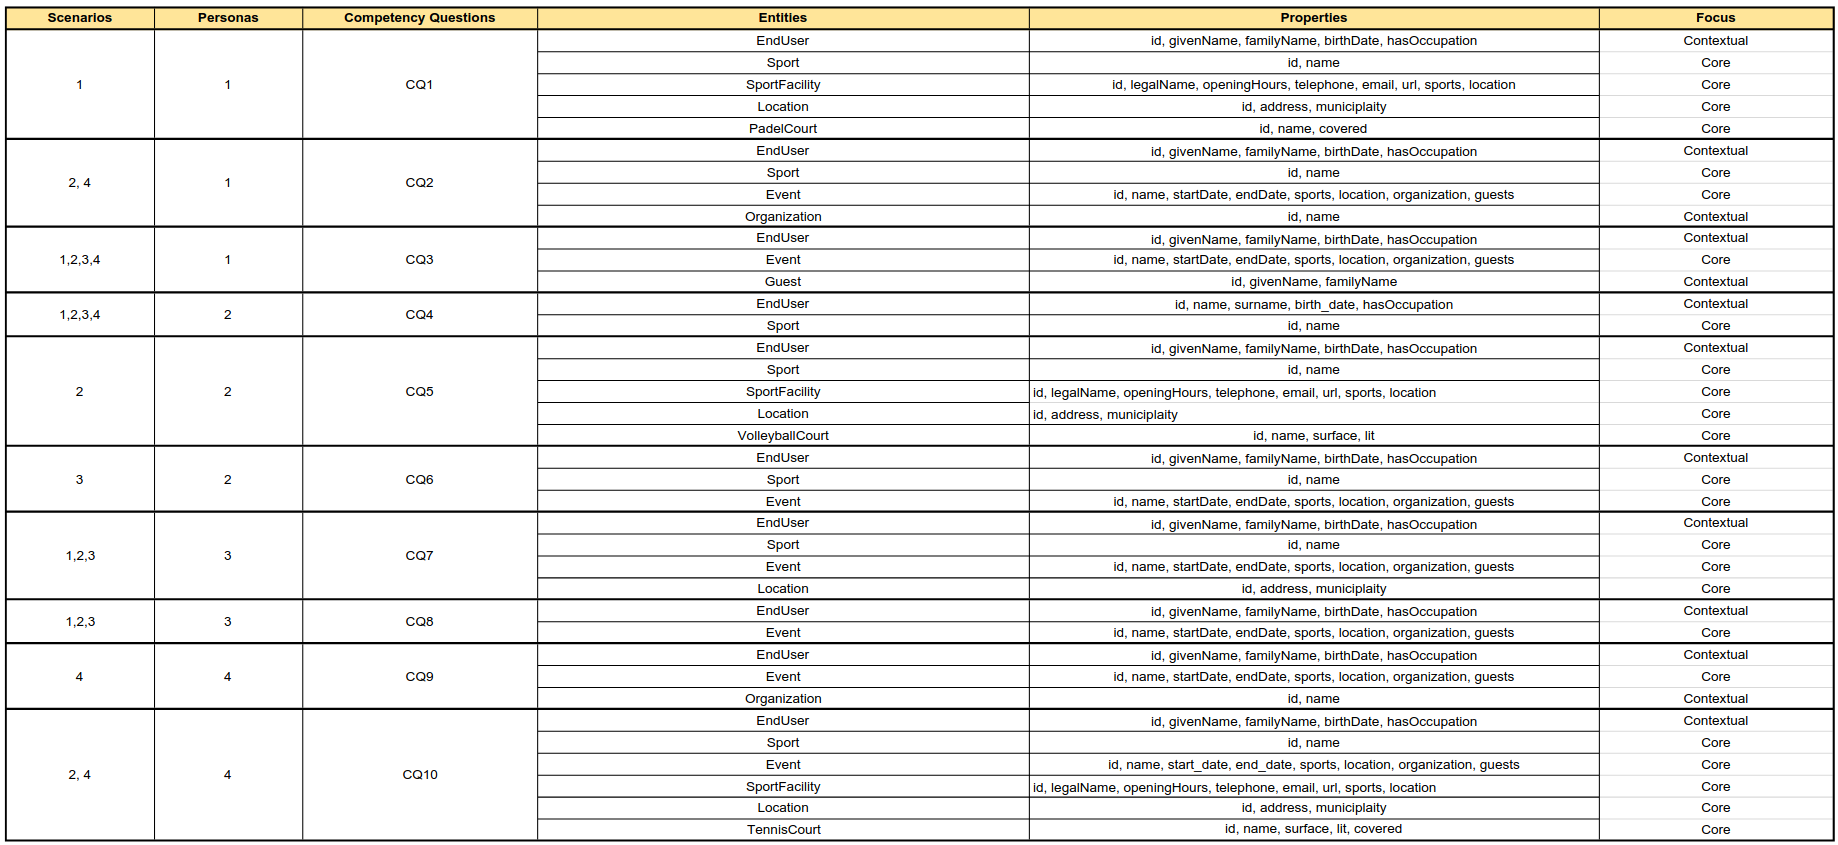
\includegraphics[width=1\linewidth]{knowdive-files/PFSheet.png}
    \caption{PF Sheet}
    \label{fig:concepts_identification}
\end{figure}

\subsection{ER model definition}
The ER diagram, which graphically represents the knowledge gathered in the prior stages. This ER diagram provides detailed information for a technician to delve deeper into the project. The diagram is based on the entity types (ETypes) and attributes identified before.
\begin{figure}[H]
    \centering
    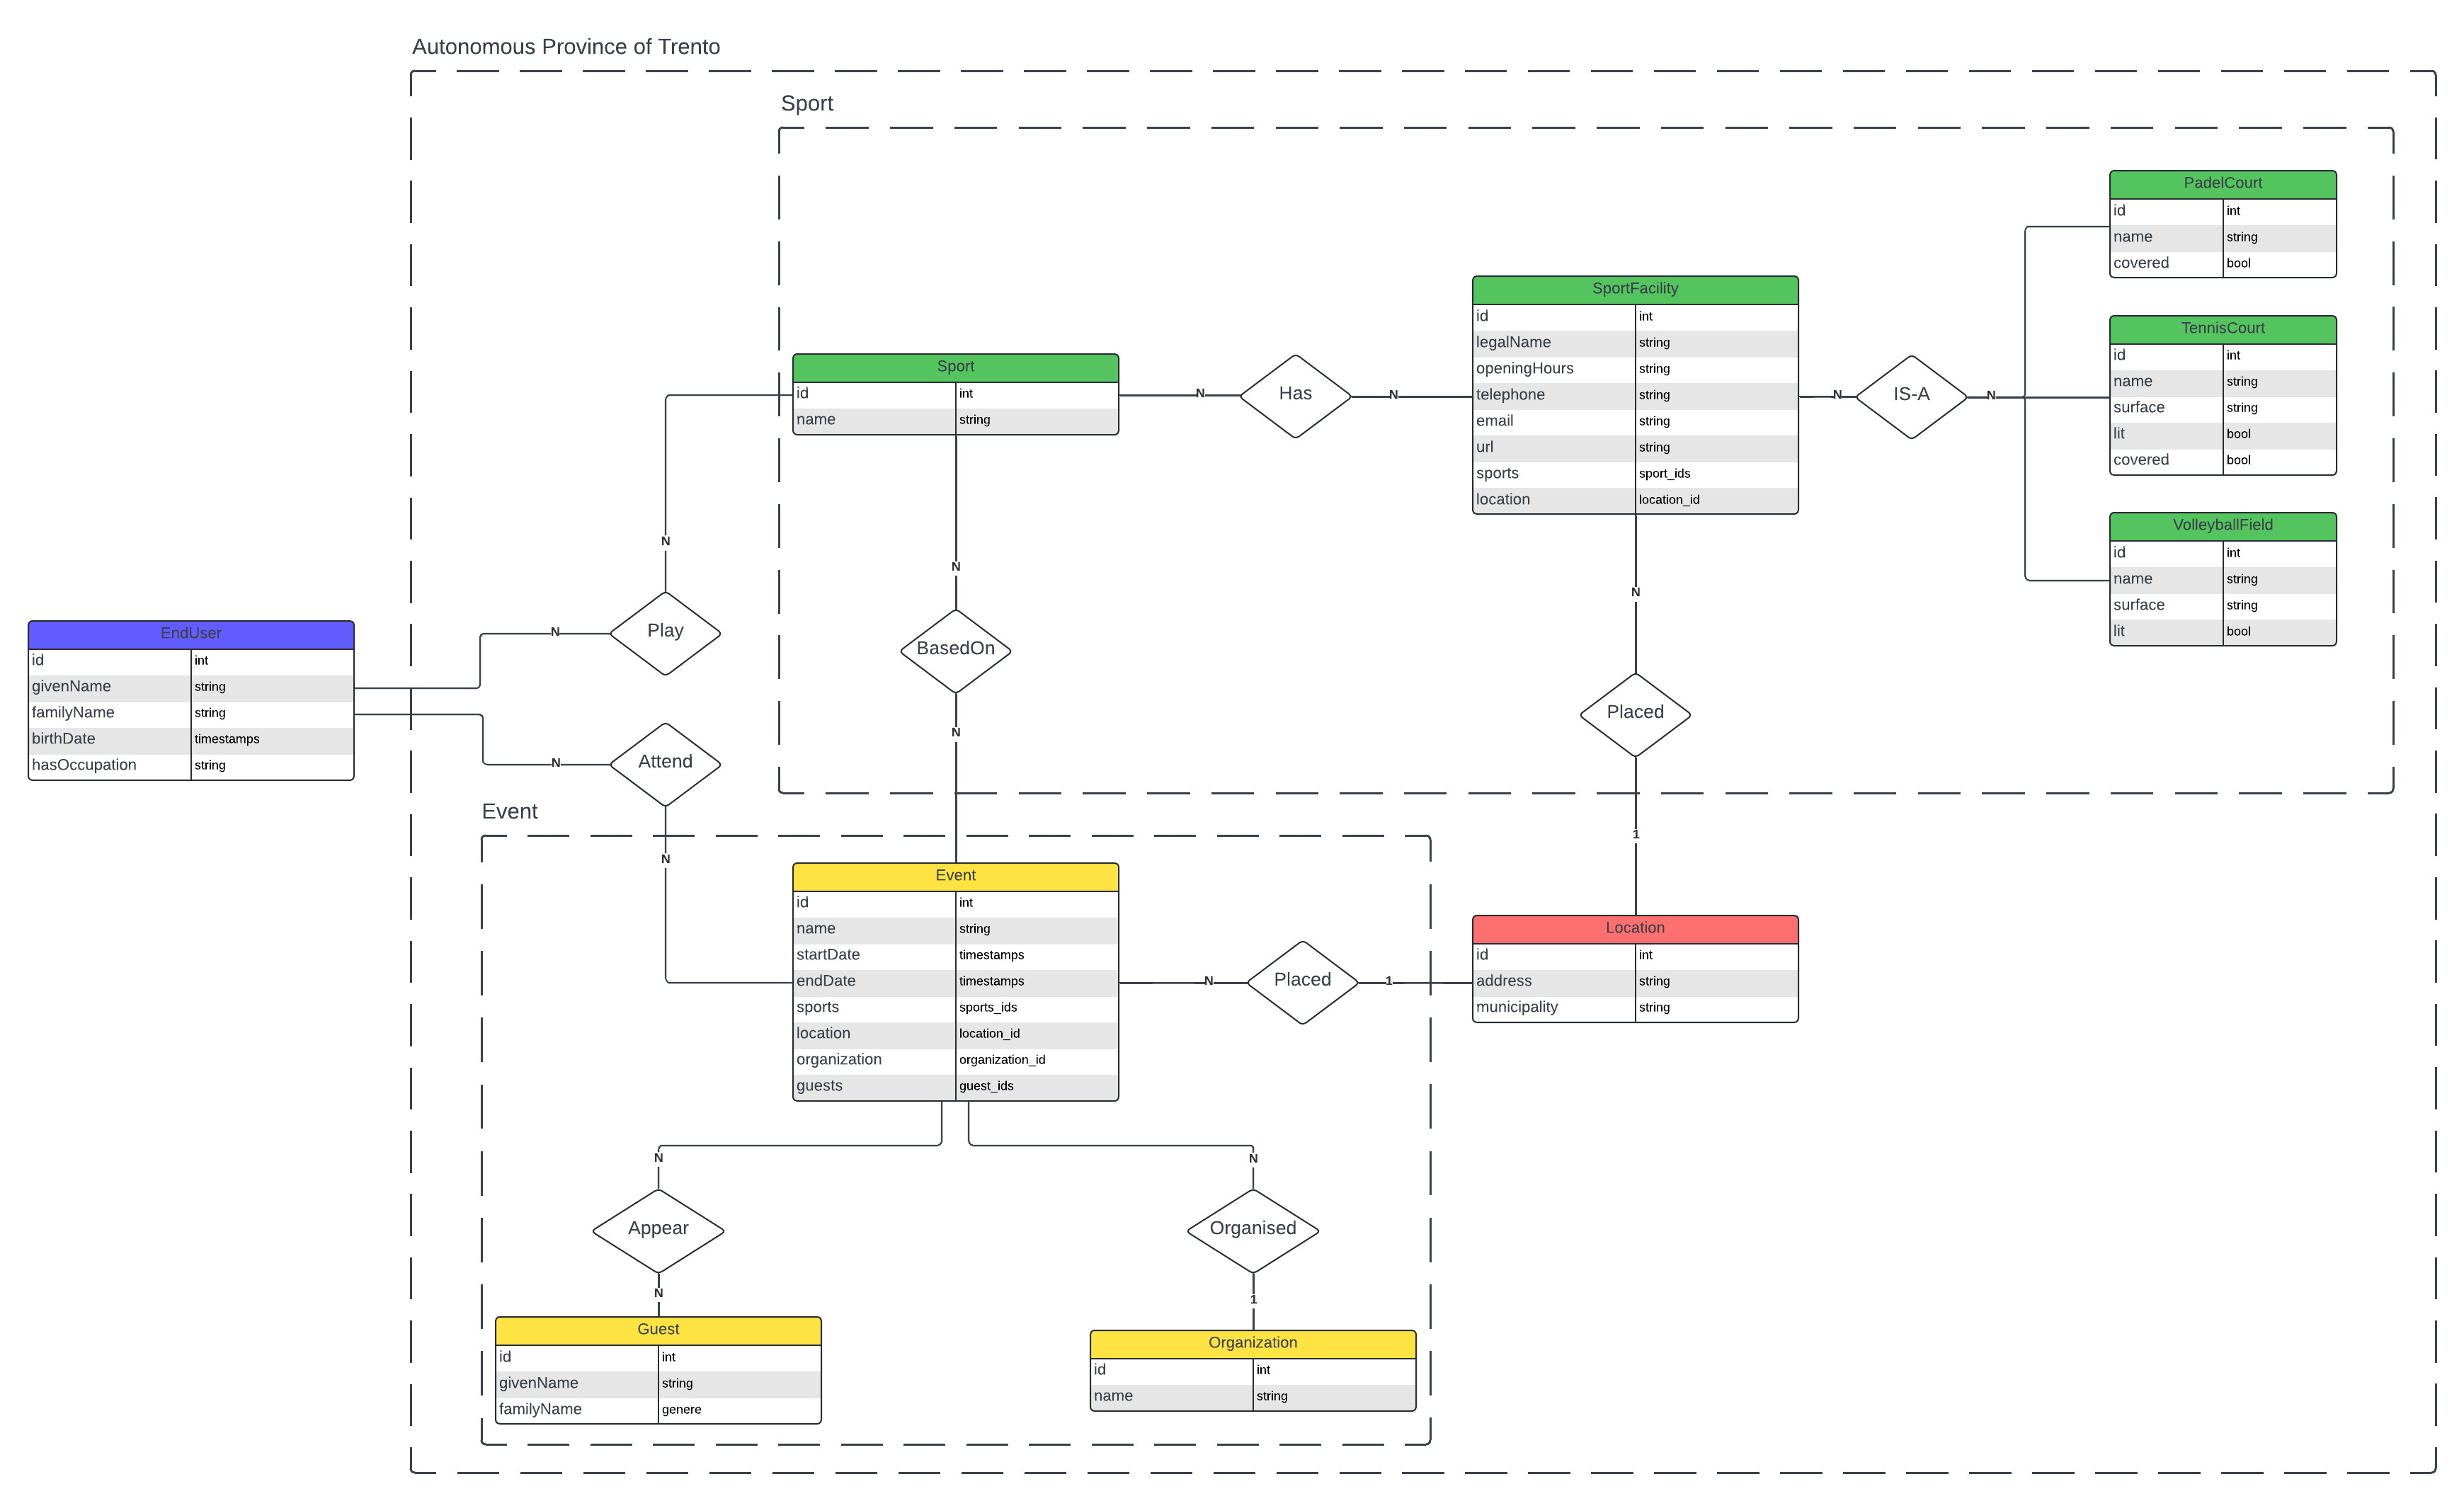
\includegraphics[width=1\linewidth]{knowdive-files/ER_model.png}
    \caption{ER model}
    \label{fig:er_model}
\end{figure}

\noindent The following ETypes shown in Figure \ref{fig:er_model} have been identified to illustrate how the different entities interact within the model, providing a clear and coherent structure for representing information about sports facilities and events in Trentino.\begin{enumerate}
    \item \textbf{SportFacility}: Represents a facility dedicated to sports, where individuals can participate in various physical activities.
    \begin{itemize}
        \item \texttt{id}: Unique identifier for each sports facility.
        \item \texttt{legalName}: Name of the sports facility.
        \item \texttt{openingHours}: Operating hours for the facility.
        \item \texttt{telephone}: Contact phone number for the facility.
        \item \texttt{email}: Contact email address for the facility.
        \item \texttt{url}: Website link for more information.
        \item \texttt{sports}: List of sports available at the facility, linked to sport IDs.
        \item \texttt{location}: Address or general location information.      
    \end{itemize}

    \item \textbf{PadelCourt}: A court dedicated to padel, a racquet sport.
    \begin{itemize}
        \item \texttt{id}: Unique identifier for the padel court.
        \item \texttt{name}: Name of the padel court.
        \item \texttt{covered}: Indicates if the court is covered.
    \end{itemize}

    \item \textbf{TennisCourt}: A court dedicated to tennis.
    \begin{itemize}
        \item \texttt{id}: Unique identifier for the tennis court.
        \item \texttt{name}: Name of the tennis court.
        \item \texttt{surface}: Type of surface on the court (e.g., clay, grass).
        \item \texttt{lit}: Indicates if the court has lighting.
        \item \texttt{covered}: Indicates if the court is covered.
    \end{itemize}

    \item \textbf{VolleyballField}: A field dedicated to volleyball.
    \begin{itemize}
        \item \texttt{id}: Unique identifier for the volleyball field.
        \item \texttt{name}: Name of the volleyball field.
        \item \texttt{surface}: Type of surface on the field (e.g., sand, grass).
        \item \texttt{lit}: Indicates if the field has lighting.
    \end{itemize}

    \item \textbf{Sport}: Represents a specific type of sport.
    \begin{itemize}
        \item \texttt{id}: Unique identifier for each sport.
        \item \texttt{name}: Name of the sport.
    \end{itemize}

    \item \textbf{Event}: Represents an organized sports event, including details on participation and scheduling.
    \begin{itemize}
        \item \texttt{id}: Unique identifier for each event.
        \item \texttt{name}: Name of the event.
        \item \texttt{startDate}: Start date of the event.
        \item \texttt{endDate}: End date of the event.
        \item \texttt{sports}: Sports included in the event, linked to sport IDs.
        \item \texttt{location}: Location where the event is held, linked to location ID.
        \item \texttt{organization}: Organization responsible for the event, linked to organization ID.
        \item \texttt{guests}: List of guest participants, linked to guest IDs.
    \end{itemize}

    \item \textbf{Guest}: Represents a guest or participant involved in a sports event.
    \begin{itemize}
        \item \texttt{id}: Unique identifier for each guest.
        \item \texttt{givenName}: The first name of the guest.
        \item \texttt{familyName}: The last name of the guest.
    \end{itemize}

    \item \textbf{Organization}: Represents an organization responsible for hosting or coordinating sports events.
    \begin{itemize}
        \item \texttt{id}: Unique identifier for each organization.
        \item \texttt{name}: Name of the organization.
    \end{itemize}

    \item \textbf{Location}: Represents a physical location where sports facilities and events are held.
    \begin{itemize}
        \item \texttt{id}: Unique identifier for each location.
        \item \texttt{address}: Full address of the location.
        \item \texttt{municipality}: City in which the location is situated.
    \end{itemize}

    \item \textbf{EndUser}: Refers to the end user who will utilize the service..
    \begin{itemize}
        \item \texttt{id}: Unique identifier for each user.
        \item \texttt{givenName}: The first name of the end user.
        \item \texttt{familyName}: The last name of the end user.
        \item \texttt{birthDate}: Birth date of the user.
        \item \texttt{hasOccupation}: The person's occupation.
    \end{itemize}
\end{enumerate}

\noindent This ER model is also structured around several relationships:
\begin{enumerate}
    \item \textbf{Placed}: It contextualizes where the facilities and events are physically situated, allowing users to identify precise addresses or areas for sports facilities and event venues.
    \item \textbf{Has}: It defines the kinds of sports activities or facilities available within each SportFacility, supporting users in finding facilities based on specific sports or equipment.
    \item \textbf{IS-A}: It allows the model to recognize these entities as specific kinds of SportFacility, enabling queries about both general facilities and specific facility types, based on shared attributes.
    \item \textbf{Organise}: It identifies the entity responsible for organizing an event, allowing users to find events hosted by specific organizations or understand the event’s affiliation.
    \item \textbf{Appear}: It enables user queries about the guest lists.
    \item \textbf{BasedOn}: Identifies the sport associated with an event.
    \item \textbf{Play}: Indicates the sport played by the user.
    \item \textbf{Attend}: Indicates the event joined by the user.
\end{enumerate}

\noindent Due to the broad accessibility of the sports world, we decided not to focus solely on the university domain; instead, we envisioned this service as accessible to everyone in Trentino. \ Building on this idea, our goal became developing a service capable of helping citizens find relevant sports events and facilities throughout Trentino.

\noindent From a temporal perspective, we chose to support requests specific to the year 2024, while from a geographical perspective, we based our service on the entire Trentino region. \\
Both these temporal and geographical choices have their strengths and weaknesses. Regarding the temporal choice, the main limitation is that we are restricted to the year 2024, as sports events data from previous years is often incomplete or inconsistent, with some years missing data entirely. Looking forward, another limitation is that our service remains fixed to 2024, as we cannot guarantee that future data providers will address these critical gaps in coverage. By focusing on 2024, however, we ensure that our service operates reliably, leveraging a dataset we know to be comprehensive—this is a major strength of our approach. \\
As for the geographical choice, as outlined in our purpose definition, our service is designed to function across the entire Trentino region, making it one of the service’s greatest strengths. However, it is important to note that for some entities, especially sports facilities, certain fields may be missing, such as contact information—particularly for less documented facilities. This also applies to specific types of facilities, such as volleyball fields, where some sports facilities may have incomplete data. Despite these gaps, we chose to model these properties because they align with the project’s purpose: providing a complete and unified view of sports facilities and events in the region. By including these attributes in the model, we establish a structure that can accommodate future data as it becomes accessible. This approach ensures that the Knowledge Graph can be expanded and refined over time, allowing it to better serve the needs of residents, tourists, and local authorities seeking information about sports opportunities in Trentino.

% ----------------------------------------------------------------------------------- %
\mycomment{
The Purpose Definition section has to report the process activities included in the first phase of the iTelos methodology, as well as the results achieved. More in details a description of the below components is required:
\begin{itemize}
    \item \textbf{Informal Purpose}: as main input for the project the initial statement describing informally the project purpose has to be reported.
    \item  \textbf{Domain of Interest (DoI)}: the domain in which the purpose is considered. The DoI has to be described in terms of space and time constraints, plus a description of its main features. The DoI description informs the reader about the geographical space, as well as the period of time, in which the project purpose is considered.
    \item \textbf{Scenarios definition}: a set of usage scenarios, describing the multiple aspects considered by the project purpose.
    \item \textbf{Personas}: a set of real users acting  within the scenarios defined above. Each Persona is defined over a specific features included in the main Purpose.  
    \item \textbf{Competency Questions (CQs)}: the list of CQs created considering the personas in the scenarios defined.
\end{itemize}

\noindent The above steps aim at catching the diversity expressed by the project purpose, by defining clearly the different aspects, about the involved contexts and actors. To this end, while describing the above activities the writer has to report those scenarios, personas and questions, whose better describe all the several and diverse aspects of the project purpose.\\

\noindent For the remaining two activities of the first iTelos phase, the writer has to specify which formal elements (entities and properties) can be extracted from the above definitions, and how they interact together with the objective of satisfying the project purpose. 
        
\begin{itemize}
    \item \textbf{Concepts identification}: the terms representing the entities, and their properties, to be consider in the KGE project, classified using the popularity categories.
    \item  \textbf{ER model definition}: the entities and property identified in the step above, are used to design the purpose ER model. this is the last step of the purpose formalization process.
\end{itemize}

\noindent The report of the work done during the first phase of the methodology, has to includes also the description of the  different choices made, with their strong and weak points. In other words the report should provide to the reader, a clear description of the reasoning conducted by all the different team members.\\
}


